\documentclass[../main.tex]{subfiles}
% !TeX root = ../main.tex
\begin{document}
	\section{Noncurrent Assets}
	
	\textbf{Non-current assets} are assets that are used actively in the 
	operations of the business, and that are expected to benefit the operations 
	into the future.
	
	There are two major categories of non-current assets:
	\begin{itemize}[noitemsep]
		\item \textbf{Tangible plant assets} are long-term assets that have 
		physical substance \eg Land, buildings, equipment, furniture, and 
		fixtures.  Land is not depreciated. Buildings, equipment, 
		furniture, and fixtures are depreciated. Depreciation allocates the 
		cost of a long-lived asset over the periods benefited by its use.
		\item \textbf{Intangible assets} are 
		long-lived assets without physical substance. Intangible assets have 
		value represented by rights that produce benefits \eg 
		Trademarks, copyrights, patents, licensing rights, technology, 
		franchises, and goodwill. Intangibles with a limited life, such as 
		patents and copyrights, are 
		subject to \textbf{amortization}. Intangibles with an unlimited (or 
		indefinite) life, such as goodwill and trademarks, are not amortized. 
		Amortization is a process of allocating cost over the useful life, 
		similar to depreciation.
	\end{itemize}
	
	\subsection{Property, Plant and Equipment (PPE)}
	The four main issues in accounting for  property, plant and equipment are:
	\begin{itemize}[noitemsep]
		\item computing the costs of  property, plant and equipment.
		\item allocating the costs of most  property, plant and equipment (less 
		any amounts of residual values) against revenues for the periods they 
		benefit.
		\item accounting for expenditures such as repairs and improvements to  
		property, plant and equipment.
		\item recording the disposal of property, plant and equipment.
	\end{itemize}

	\begin{figure}[ht]
		\centering
		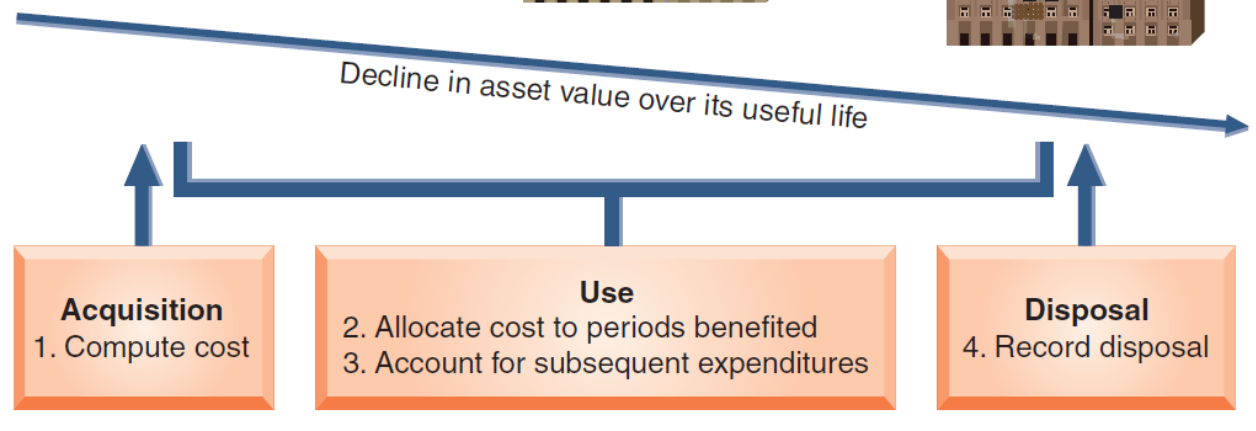
\includegraphics[width=\columnwidth]{images/c8/ppe_costs.png}
	\end{figure}
	
	\subsubsection{Acquisition Cost}
	
	The \textbf{acquisition cost} of an item of property, plant and equipment 
	includes the purchase price as well as all costs necessary to get the asset 
	in place and ready for its intended use. We record the purchase price net 
	of any cash discounts available. We will add freight, unpacking, 
	assembling, installing, and testing costs to the net invoice price to 
	arrive at the final cost.
	
	Finance charges are not included in the cost of an asset. If we elect to 
	finance the purchase over a period of time, the interest cost is charged as 
	an expense when incurred.
	
	\paragraph{Land.} Land is not a depreciable asset. In addition to the 
	purchase price, there 
	are many costs generally incurred in connection with the acquisition. Many 
	of these costs are related to obtaining legal title to the land.
	
	\paragraph{Land Improvements.} Land improvements are depreciated over their 
	useful life. Land improvements 
	include parking lots, driveways, fences, sidewalks, landscaping, and any 
	outdoor lighting systems.
	
	While the costs of these improvements increase the usefulness of the land, 
	they are charged to a separate \textbf{Land Improvement account} so that 
	their costs 
	can be allocated to the periods they benefit.
	
	\paragraph{Building.} Whether we purchase or construct a building, the cost 
	should include the purchase price plus any attorney fees or title fees. If 
	we construct the building, the cost will include all the necessary 
	construction costs as well as the costs just mentioned.
	
	\paragraph{Machinery and Equipment.} The costs of machinery and equipment 
	consist of all costs normal and necessary to purchase them and prepare them 
	for their intended use. These include the purchase price, taxes, 
	transportation charges, insurance while in transit, and the installing, 
	assembling, and testing of the machinery and equipment.
	
	\subsubsection{Lump-sum Asset Purchase}
	
	In lump-sum asset purchase, the total cost of a combined purchase of land 
	and building is separated on the basis of their relative market values.
	
	\begin{figure}[ht]
		\centering
		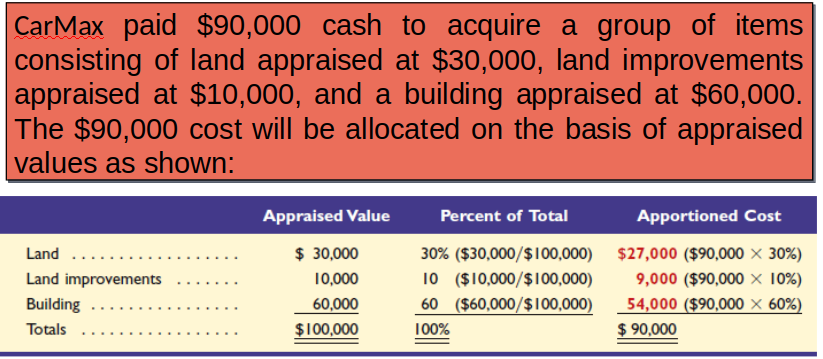
\includegraphics[width=\columnwidth]{images/c8/lump_sum_purchase_eg.png}
	\end{figure}
	
	\subsection{Depreciation}
	
	\textbf{Depreciation} is a process of cost allocation. We allocate the cost 
	of the asset to expense over its useful life in some rational and 
	systematic manner. 
	
	The unused portion of the asset’s cost appears on the statement of 
	financial position. We allocate a portion of the cost to expense on the 
	income statement each accounting period.
	
	The calculation of depreciation requires three amounts for each asset:
	\begin{itemize}[noitemsep]
		\item the asset’s \textbf{cost};
		\item he estimated \textbf{residual value} we expect to receive at the 
		end of its useful life
		\item the estimated \textbf{useful life} of the asset. This is the 
		amount the owner expects to receive when disposing of the asset. The 
		useful life of an item of property, plant and equipment is the length 
		of time it is productively used in a company’s operations.
	\end{itemize}
	 Once these three amounts are known, we select the depreciation method that 
	 we will use to calculate depreciation expense. There are three popular 
	 methods of calculating depreciation expense:
	 \begin{itemize}[noitemsep]
	 	\item \textbf{Straight-line}
	 	\item \textbf{Units-of-production} - charges a varying amount to 
	 	expense for each period of an asset’s useful life depending on its 
	 	usage.
	 	\item \textbf{Declining Balance} - we take more depreciation expense in 
	 	the early years of the asset’s life and lower amounts of depreciation 
	 	in later years. Several profit-tax depreciation calculations are based 
	 	on the declining balance method. 
	 \end{itemize}
	 
	\subsubsection{Straight-line Depreciation}
	\begin{figure}[ht!]
		\centering		
		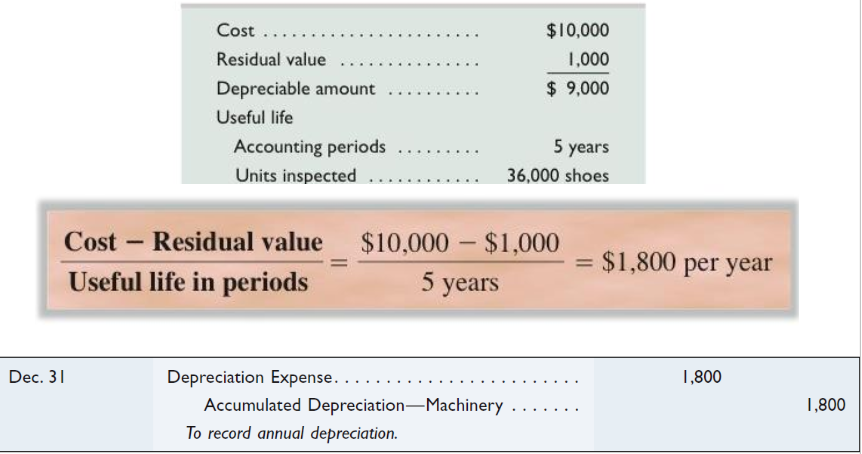
\includegraphics[width=\columnwidth]{images/c8/straight_line_eg.png}
	\end{figure}
	Straight-line Depreciation expense for any given period is determined by 
	taking the asset’s cost less its estimated residual value and dividing this 
	amount by 
	the asset’s estimated useful life. If we calculate annual depreciation, we 
	would express the useful life in years.
	
	Accumulated depreciation is subtracted from the cost of the asset to arrive 
	at what is called \textbf{carrying amount}. The carrying amount is the 
	amount shown on the statement of financial position.

	\begin{figure}[ht!]
		\centering		
		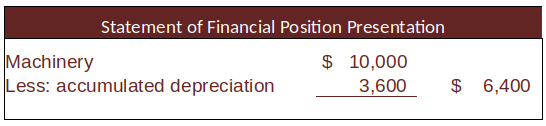
\includegraphics[width=.8\columnwidth]{images/c8/straight_line_fp_eg.png}
		\caption{Statement of Financial Position Presentation}
	\end{figure}
	
	Note these three points for straight-line depreciation:
	\begin{itemize}[noitemsep]
		\item Depreciation expense is the same each period.
		\item Accumulated depreciation is the sum of current and prior periods’ 
		depreciation expense.
		\item Carrying amount declines each period until it equals residual 
		value at the end of the machine’s useful life.
	\end{itemize}
	
	\subsubsection{Units of Production}
	Under the units-of-production method, the first step is to calculate the 
	depreciation expense per unit of production. Take the asset’s cost less its 
	residual value and divide this amount by the total estimated number of 
	units that will be produced by the assets.
	
	\begin{figure}[ht!]
		\centering		
		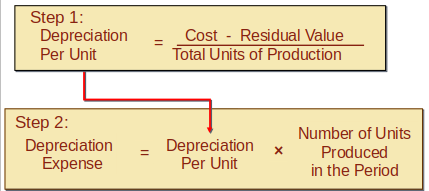
\includegraphics[width=.8\columnwidth]{images/c8/depreciation_uop.png}
		\caption{Units-of-Production}
	\end{figure}

 	Once we complete the first step, 
	we may calculate depreciation expense for the period. Multiply the 
	depreciation expense per unit that we determined in step one by the number 
	of units produced in the current period.

	\begin{figure}[ht!]
		\centering		
		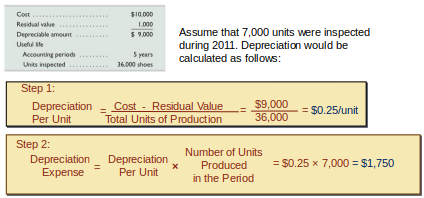
\includegraphics[width=1\columnwidth]{images/c8/uop_eg.png}
	\end{figure}

	Units of Production Depreciation show that:
	\begin{itemize}[noitemsep]
		\item Depreciation expense depends on unit output.
		\item Accumulated depreciation is the sum of current and prior periods’ 
		depreciation expense.
		\item Carrying amount declines each period until it equals residual 
		value at the end of the asset’s useful life.
	\end{itemize}

	\subsubsection{Double-Declining-Balance Method}
	
	\textbf{Declining-balance methods} yield larger depreciation expense in the 
	early years of an asset’s life and less depreciation in later years. The 
	most popular declining-balance method is called \textbf{double-declining 
	balance (DDB) method}. This method has three steps:
	\begin{enumerate}[noitemsep]
		\item Calculate the straight-line depreciation rate. 
		\item Calculate the double-declining-balance rate. We do this by 
		multiplying the straight-line rate times two.
		\item Calculate depreciation expense. We multiply the double-declining 
		rate times the carrying amount of the asset at the beginning of the 
		period. Recall that carrying amount is equal to cost less accumulated 
		depreciation. Under the double-declining-balance method, we ignore 
		estimated residual value (remember, carrying amount is equal to the 
		cost of the asset minus the accumulated depreciation). Don’t forget 
		that residual value is not used in the double-declining-balance method. 
		We base depreciation expense on the carrying amount of the asset at the 
		beginning of the year.
	\end{enumerate}
	
	\begin{figure}[ht!]
		\centering		
		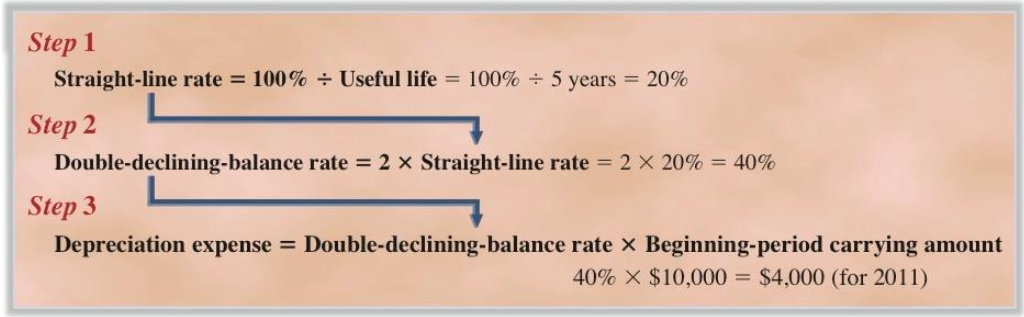
\includegraphics[width=1\columnwidth]{images/c8/ddb_method.png}
	\end{figure}

	We always want the carrying amount to be equal to estimated residual value 
	at the end of the asset’s useful life, but it just will not work properly 
	using the double-declining-balance method. So in the last year of the 
	asset’s useful life, we must determine the depreciation expense necessary 
	to make the carrying amount equal to residual value.

	\subsubsection{Partial-Year Depreciation}
	
	When an item of property, plant and equipment is acquired during the year, 
	depreciation is calculated for the fraction of the year the asset is owned.
	
	\begin{figure}[ht]
		\centering
		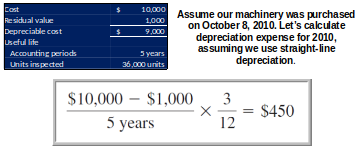
\includegraphics[width=\columnwidth]{images/c8/partial_year_depreciation.png}
	\end{figure}
	
	\subsubsection{Changes in Estimates for Depreciation}
	
	Depreciation is based on estimates of residual value and useful life. 
	During the useful life of an asset, new information may indicate that these 
	estimates are inaccurate.

	If our estimate of an asset’s useful life and/or residual value changes, 
	use the new estimate to compute depreciation for current and future 
	periods. This means that we revise the depreciation expense computation by 
	spreading the cost yet to be depreciated over the remaining useful life. 
	This approach is used for all depreciation methods.

	\begin{figure}[ht]
		\centering
		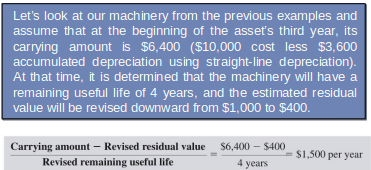
\includegraphics[width=\columnwidth]{images/c8/change_depreciation_estimate_revision_eg.png}
	\end{figure}
	
	\subsubsection{Reporting Depreciation}
	
	Both the cost and accumulated depreciation of  property, plant and 
	equipment are reported on the statement of financial position or in its 
	notes. For most companies, total accumulated depreciation is subtracted for 
	the total cost of property, plant, and equipment.
	
	\begin{figure}[ht]
		\centering
		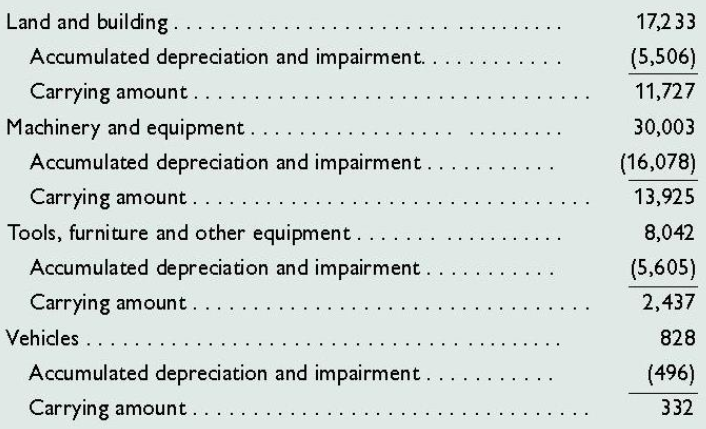
\includegraphics[width=\columnwidth]{images/c8/reporting_depreciation.png}
		\caption{Reporting Depreciation}
	\end{figure}

	\subsubsection{Revenue and Capital Expenditures}
	
	After an item of property, plant and equipment is purchased, the company 
	may incur additional expenditures on that asset. These expenditures may be 
	for repairs and maintenance, overhauls, upgrading the asset, and similar 
	expenditures. In recording these expenditures, it must decide whether to 
	capitalize or expense them (to capitalize an expenditure is to debit the 
	asset account). The issue is whether these expenditures are reported as 
	current period expenses or added to the asset’s cost and depreciated over 
	its remaining useful life.
	
	One way to handle these types of expenditures is to treat them as a capital 
	expenditure and charge the amount to a statement of financial position 
	account like the asset or accumulated depreciation. In most cases, the 
	capital expenditure represents an additional cost of  property, plant and 
	equipment that provide benefits extending beyond the current period. In 
	some cases, the expenditures may be treated as a revenue expenditure and 
	charged to current period profit as an expense. For each expenditure 
	subsequent to acquisition of an item of property, plant and equipment, we 
	must decide if the expenditure is to be treated as a capital or revenue 
	expenditure.
	
	
	\begin{figure}[ht]
		\centering
		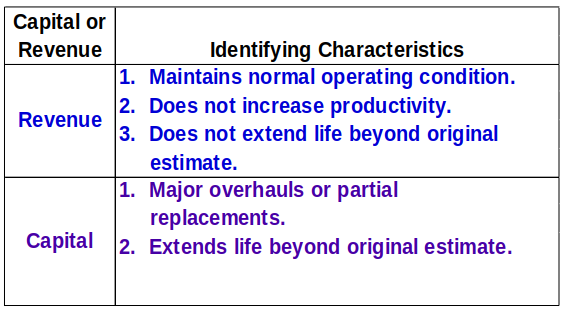
\includegraphics[width=.8\columnwidth]{images/c8/revenue_or_capital.png}
		\caption{Revenue or Capital}
	\end{figure}
	
	Generally, subsequent expenditures for ordinary repairs are treated as 
	revenue expenditures and charged to current period profit as an expense. 
	Subsequent expenditures that are major ovehauls or partial replacements or 
	extends life beyond original estimate should be treated as capital 
	expenditures and charged to the asset account.
	
	\subsubsection{Additional Expenditure}
	
	If the amounts involved are not material, most companies expense the item


	\begin{figure}[ht]
		\centering
		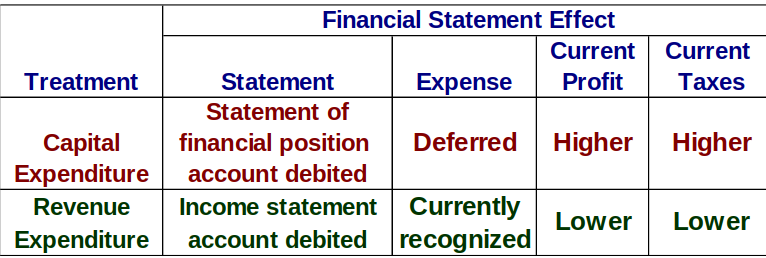
\includegraphics[width=1\columnwidth]{images/c8/additional_expenditures.png}
	\end{figure}

	\subsection{Measurement Models}
	
	IAS 16 allows a reporting entity to choose either the cost model or the 
	revaluation model and apply that policy to an entire class of property, 
	plant and equipment.
	
	\subsubsection{Cost Model}
	
	This model states that after recognition as an asset, an 
	item of property, plant and equipment shall be carried at its cost less any 
	accumulated depreciation and any accumulated impairment losses.
	
	\subsubsection{Revaluation Model}
	
	This model states that after recognition as an asset, an item of property, 
	plant and equipment whose fair value can be measured reliably shall be 
	carried at a revalued amount, being its fair value at the date of the 
	revaluation less any subsequent accumulated depreciation and subsequent 
	accumulated impairment losses. The fair value of property, plant and 
	equipment is usually determined from market-based evidence by professional 
	appraisal or valuation.
	
	\begin{figure}[ht]
		\centering
		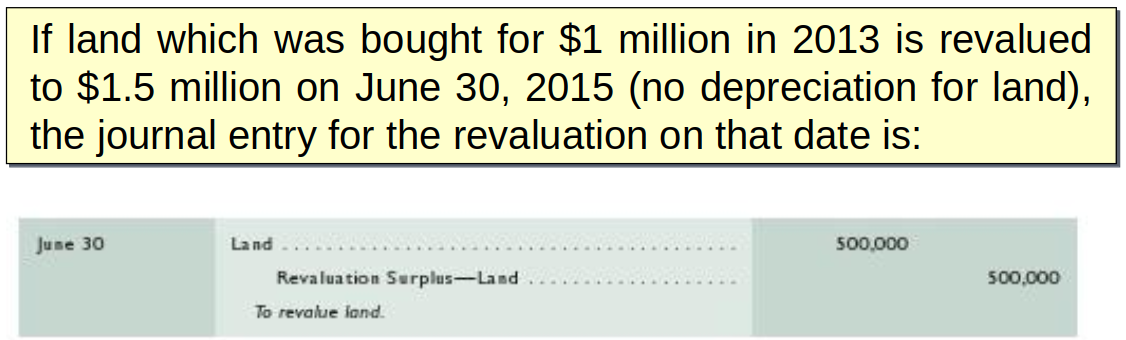
\includegraphics[width=1\columnwidth]{images/c8/revaluation_eg.png}
	\end{figure}

	\textbf{Revaluation surplus/reserve} is part of other comprehensive income.
	
	\subsubsection{Impairment}
	
	 A reporting entity has to calculate its assets’ carrying amounts, which 
	 are  after deducting any accumulated depreciation (amortization) and 
	 accumulated impairment losses. An \textbf{impairment} is the amount by 
	 which the carrying amount of an asset exceeds its recoverable amount.
	
		
	\begin{figure}[ht]
		\centering
		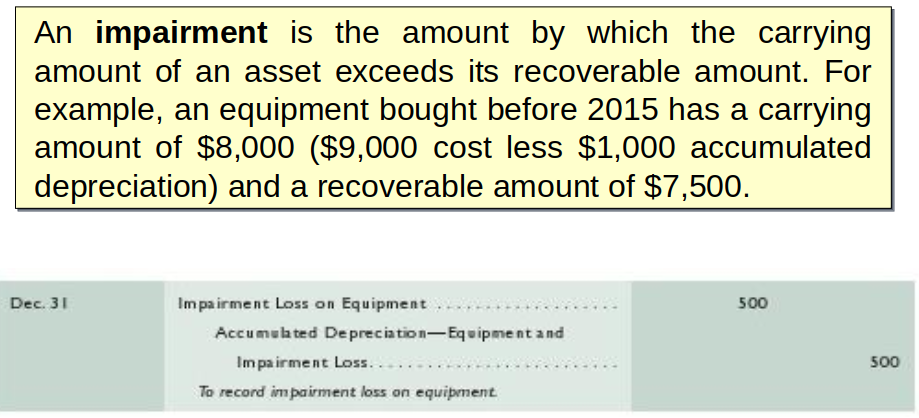
\includegraphics[width=1\columnwidth]{images/c8/impairment_eg.png}
	\end{figure}
	
	
	\subsection{Disposal of Property, Plant and Equipment}
	
	Whenever we dispose of an item of property, plant and equipment, the first 
	thing we do is update depreciation to the date of disposal. 
	After 
	completing the update, we can prepare the journal entry. We do so by 
	recording a debit to the cash account, if cash was received, or credit the 
	cash account, if cash was paid by the company. 
	
	\begin{figure}[ht]
		\centering
		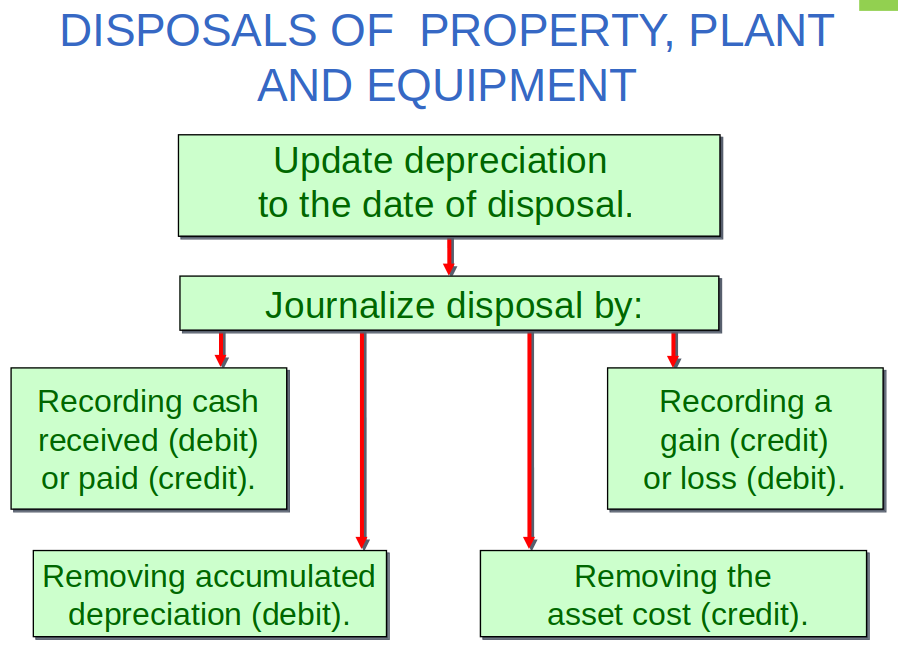
\includegraphics[width=1\columnwidth]{images/c8/disposal.png}
	\end{figure}
	
	In addition, we must 
	determine whether a gain or loss is associated with the disposal. A gain is 
	recorded with a credit, just like revenue, and a loss is recorded with a 
	debit, just like an expense account. We complete the entry by removing the 
	asset’s cost from our books with a credit, and remove the related 
	accumulated depreciation with a debit.
	\begin{itemize}[noitemsep]
		\item If the amount of cash received is greater than the carrying 
		amount of the asset (cost less accumulated depreciation), a gain is 
		associated with the disposal.
		\item If the cash received is less than the carrying amount of the 
		asset, a loss will be recorded.  
		\item When the amount of cash is exactly equal to the carrying amount 
		of the asset, there will be no gain or loss in connection with the 
		disposal.
	\end{itemize}

	\begin{figure}[ht]
		\centering
		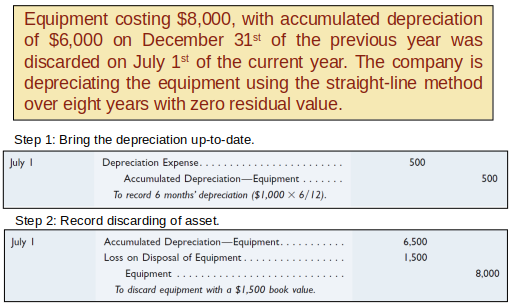
\includegraphics[width=1\columnwidth]{images/c8/discard_eg1.png}
		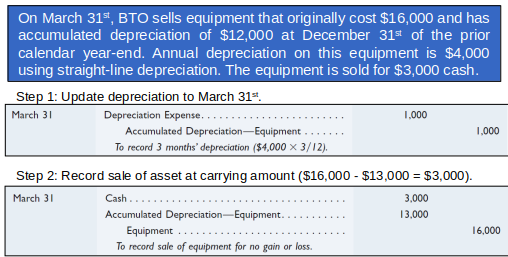
\includegraphics[width=1\columnwidth]{images/c8/discard_eg2.png}
		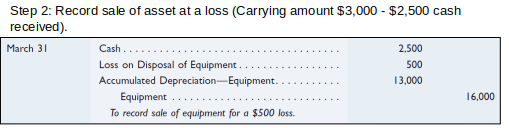
\includegraphics[width=1\columnwidth]{images/c8/discard_eg3.png}	
	\end{figure}

	\subsection{Intangible Assets}
	
	Intangible assets \eg patents, copyright, franchises and licenses, 
	goodwill, trademark and trade names, lack physical substance and that makes 
	it difficult 
	to 
	determine the asset’s useful life or any residual value. Many intangible 
	assets involve exclusive rights or privileges.
	
	Intangible assets are normally recorded at the purchase price plus any 
	legal or related fees. Intangible assets with limited lives should be 
	amortized over the period benefited using the straight-line method. 
	Intangible assets with unlimited lives should be carried at unimpaired 
	value. There should be an annual evaluation of the intangible asset to make 
	sure that there has been no impairment in value.
	
	
\end{document}